\section{Reconstruction d'images}
\subsection{Acquistion d'images}
\begin{frame}{Acquisition d'images}
    % Première image
    \only<1>{
        \begin{block}{Système de vision humaine}
            \begin{figure}
                \centering
                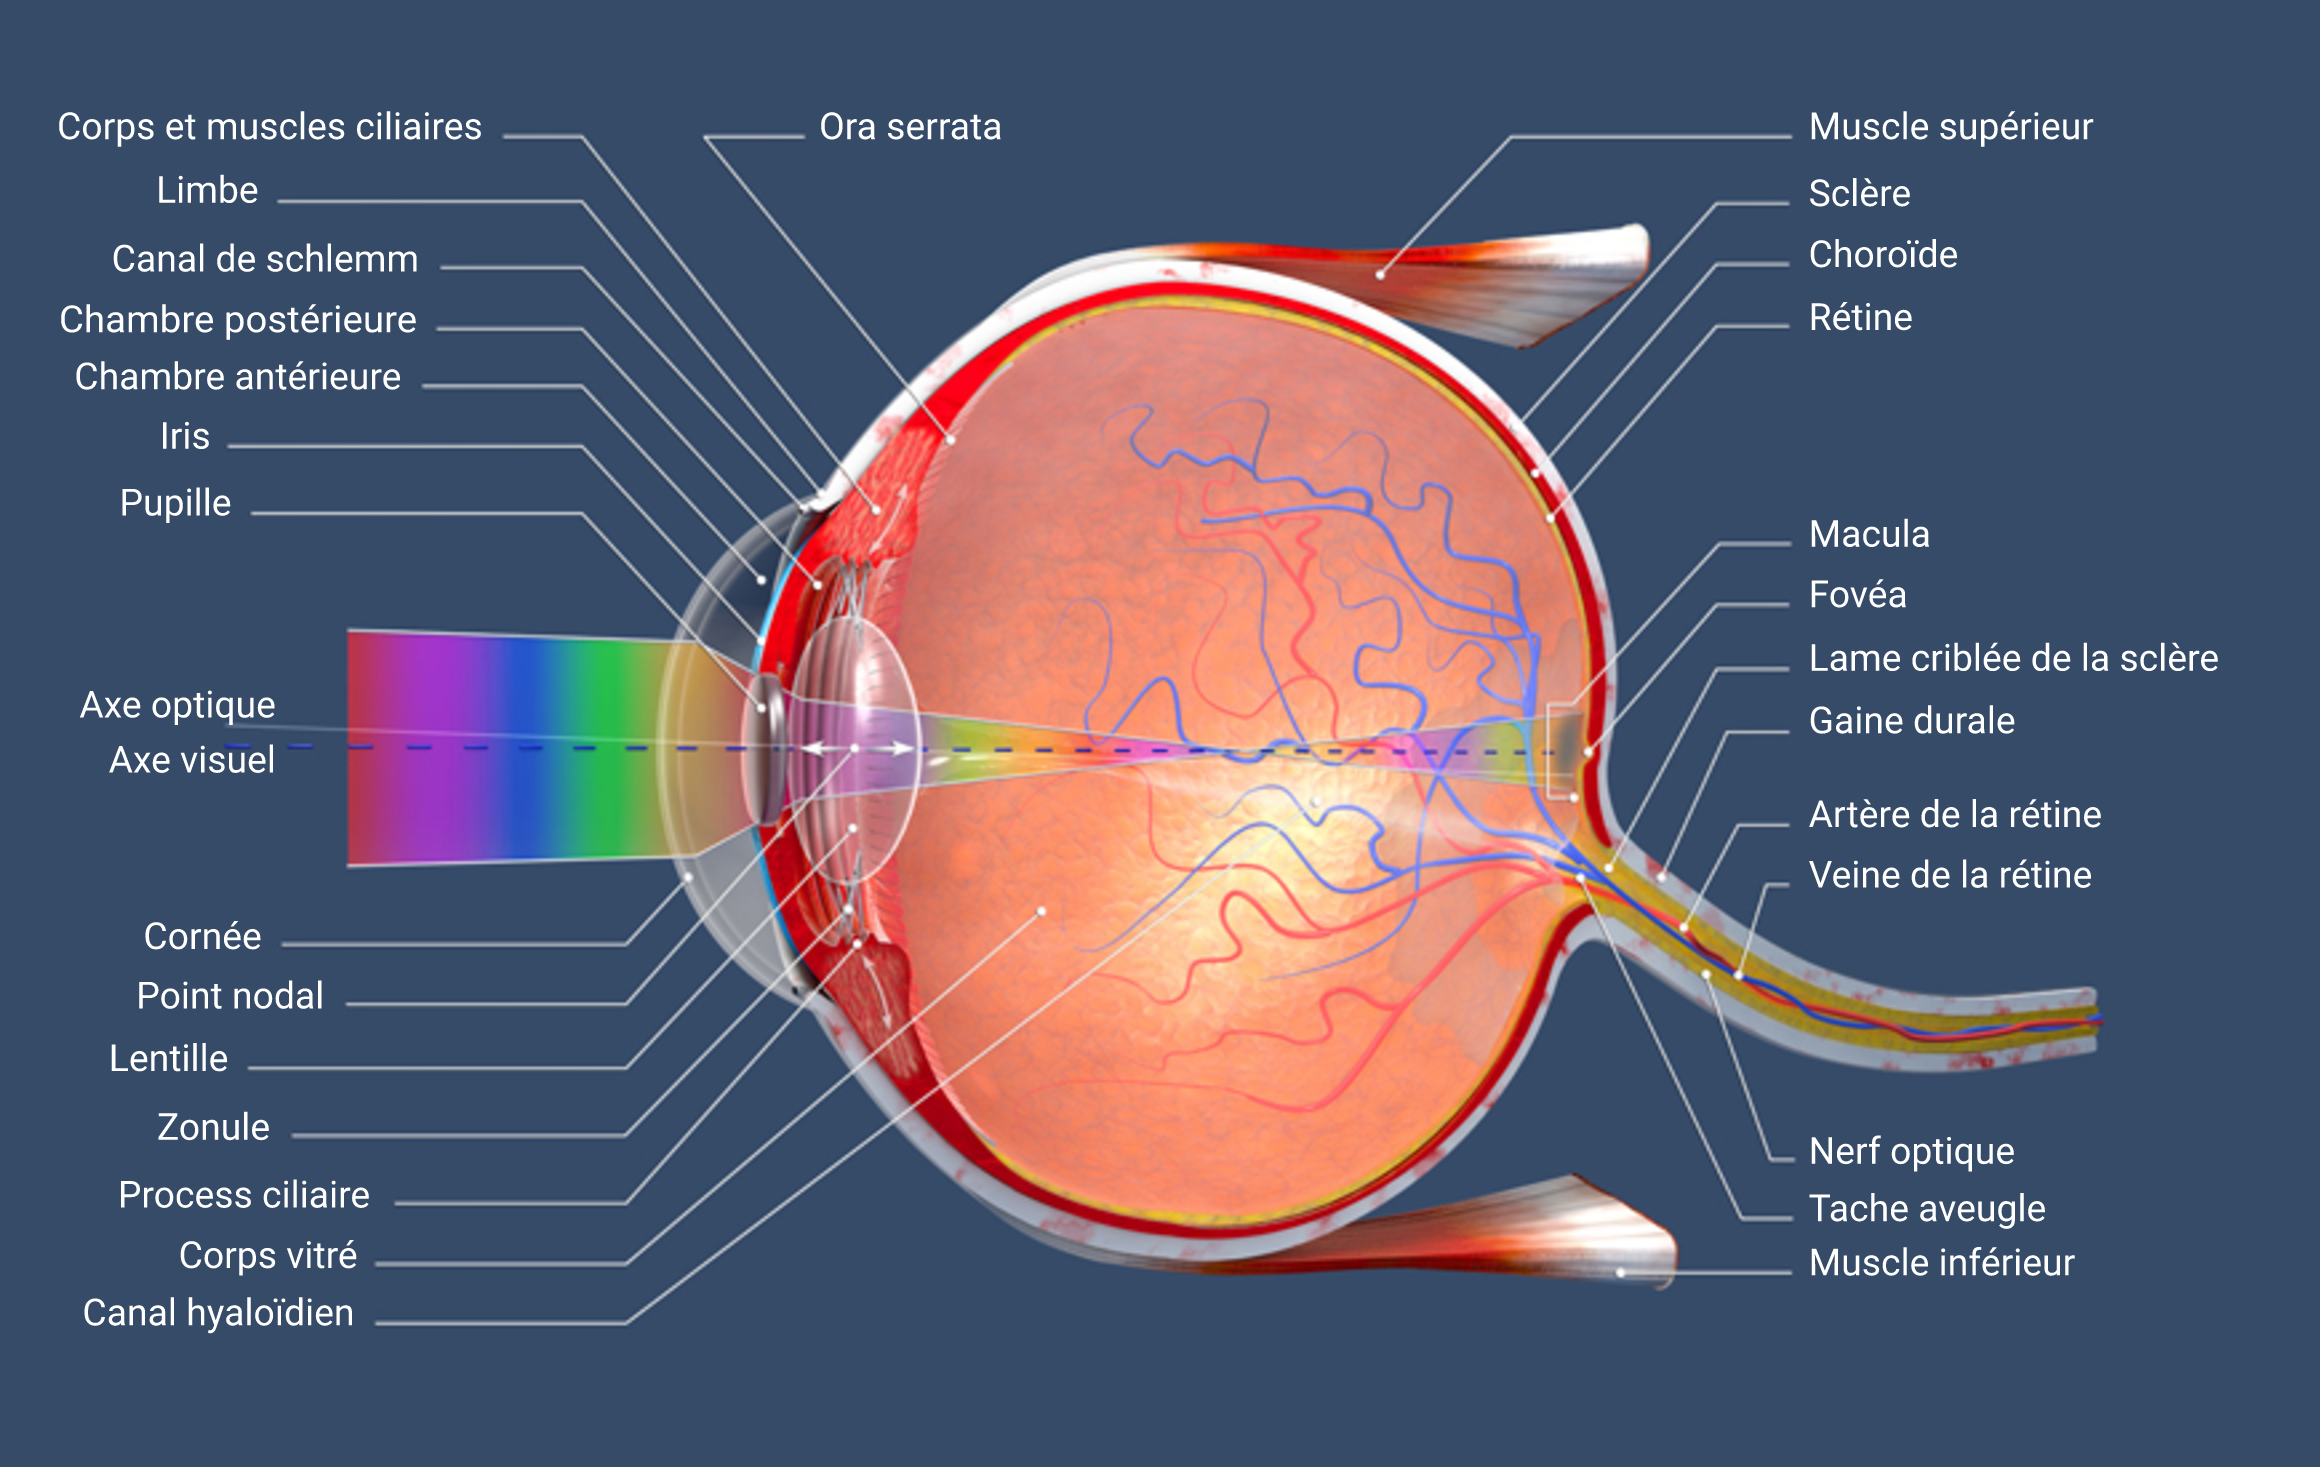
\includegraphics[width=0.6\textwidth]{../images/eye.png}
                \caption{Anatomie de l'œil humain}
                \label{fig:eye_human}
            \end{figure}
        \end{block}
    }
    % Deuxième image
    \only<2>{
        \begin{block}{Acquisition d'images analogique}
            \begin{figure}
                \centering
                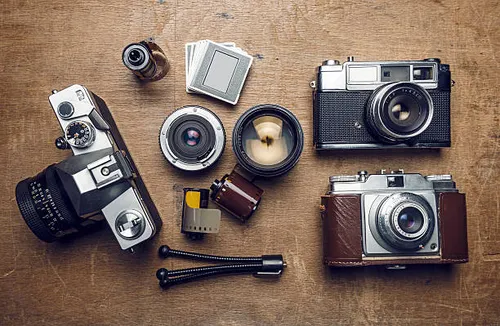
\includegraphics[width=0.6\textwidth]{../images/analog_photo.png}
                \caption{Photographie argentique -- appareils photo analogiques}
                \label{fig:analog_photo}
            \end{figure}
        \end{block}
    }
    % Troisième image
    \only<3>{
        \begin{block}{Acquisition d'images numérique}
            \begin{figure}
                \centering
                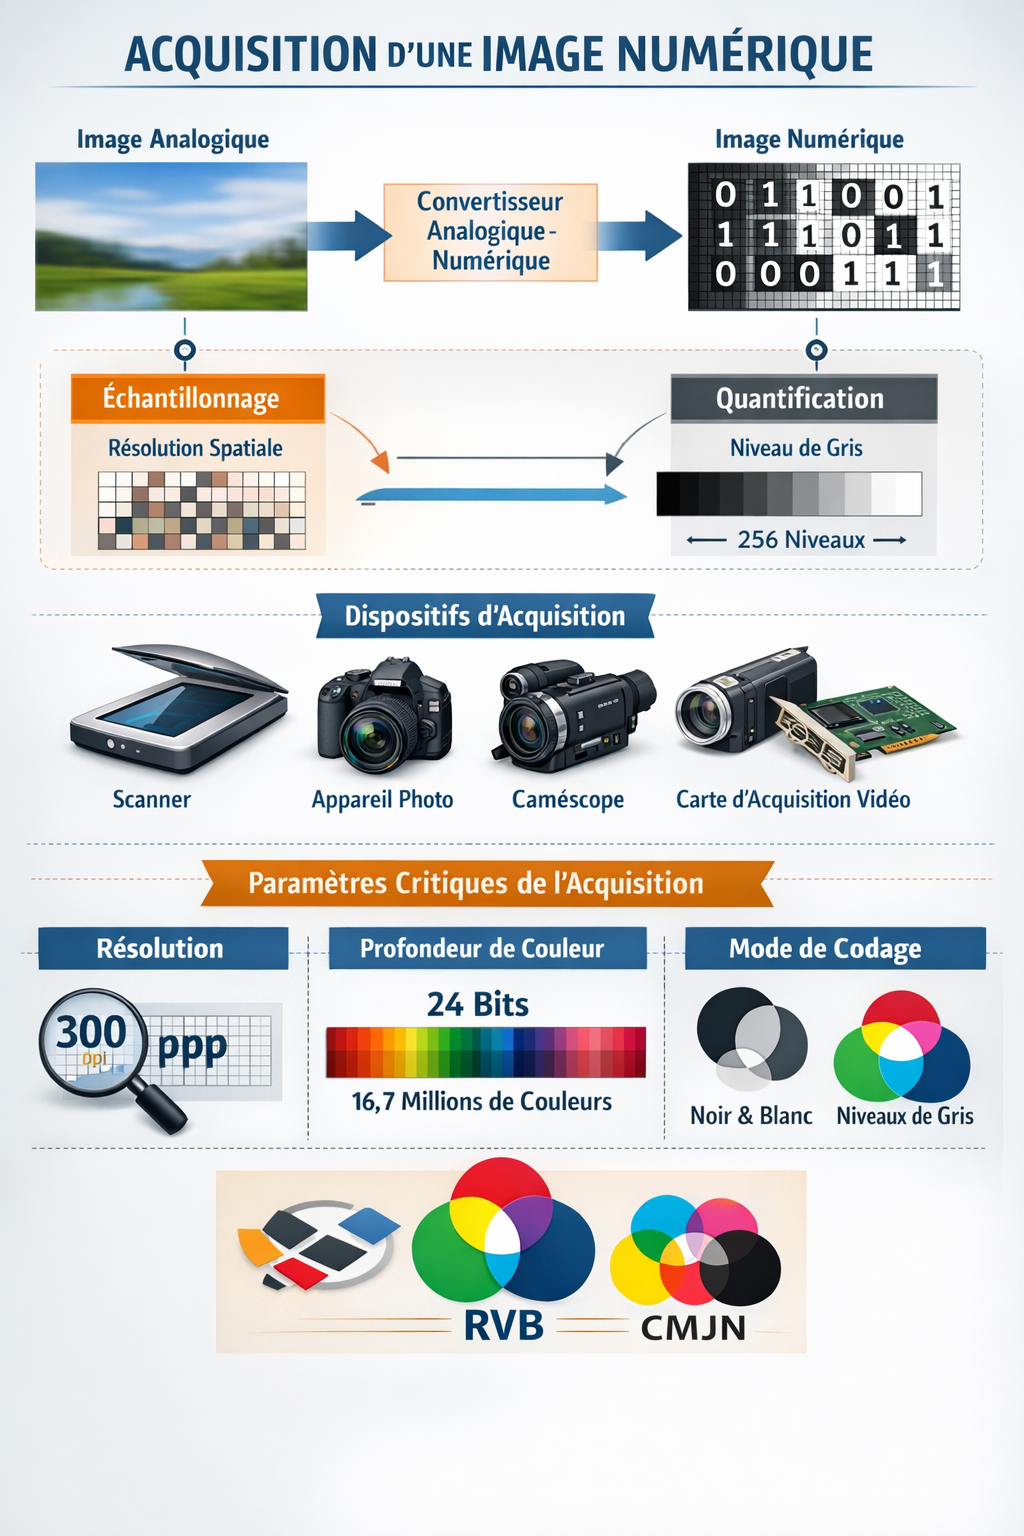
\includegraphics[height=6cm, keepaspectratio]{../images/numerical_image.png}
                \caption{Image numérique}
                \label{fig:numeric_image}
            \end{figure}
        \end{block}
    }
\end{frame}
\subsection{Système de reconstruction}
\begin{frame}{Transformation des mesures brutes en image diagnostique}
    \begin{columns}
    \column{0.5\textwidth}
    \begin{block}{Problématique}
        \begin{itemize}
            \item Les capteurs (TDM, IRM, TEP) ne mesurent \textbf{pas directement} l'image.
            \item Les données brutes $y$ sont \textbf{partielles, indirectes et bruitées}.
            \item Objectif : estimer l'image inconnue $x$ à partir de $y$.
            $\Rightarrow$ Problème \textbf{inverse}, généralement \textbf{mal posé} (non-unicité, instabilité).
        \end{itemize}
    \end{block}

    \column{0.5\textwidth}
    \begin{block}{Modélisation mathématique}
        \begin{equation}
            y = Hx + n
        \end{equation}
        \begin{itemize}
            \item $x$ : image à reconstruire (inconnue)
            \item $H$ : opérateur direct (modélise la physique de l'acquisition)
            \item $n$ : bruit de mesure
            \item $y$ : mesures acquises (sinogramme, espace $k$, projections)
        \end{itemize}
    \end{block}
\end{columns}
\end{frame}

\subsection{Algorithmes de reconstruction}
\begin{frame}{Algorithmes de reconstruction}
% Block FBP
    \only<1>{\begin{block}<1>{Rétroprojection filtrée (FBP)}
        \begin{itemize}
            \item Basée sur la transformée inverse de Radon
            \item Rapide et largement utilisée en CT et TEP
            \item Limites et artefacts :
                \begin{itemize}
                    \item Amplification du bruit
                    \item Artefacts de stries et anneaux
                    \item Sensible aux mouvements et données incomplètes
                \end{itemize}
        \end{itemize}
    \end{block}}

    \only<2>{\begin{block}{Compressive Sensing (CS)}
        \begin{itemize}
            \item Exploite la parcimonie des images médicales
            \item Reconstruction à partir de moins de mesures → réduction dose et temps d’acquisition
            \item Algorithmes itératifs avec régularisation pour limiter bruit et artefacts
            \item Limites et artefacts :
                \begin{itemize}
                    \item Sensible au choix de la base parcimonieuse et hyperparamètres
                    \item Artefacts spécifiques : blocs, textures irrégulières, effet staircasing
                \end{itemize}
            \item Stratégies d’amélioration :
                \begin{itemize}
                    \item Optimisation du sous-échantillonnage et des acquisitions
                    \item Algorithmes itératifs avancés (ex. ADMM)
                    \item Post-traitement : filtrage, amélioration du contraste
                    \item Approches hybrides : modèles physiques + statistiques
                \end{itemize}
        \end{itemize}
    \end{block}}

\end{frame}